\section{Wdrożenie aplikacji}

W celu dostosowania aplikacji do środowiska produkcyjnego wykorzystano usługi chmury Microsoft Azure. Operacja ta miała na celu znalezienie i eliminację błędów, które mogą się pojawić na nowym serwerze. Umożliwiło to skorzystanie z niej z publicznego adresu sieci WWW oraz wykonanie testów na środowisku innym niż programistyczne. 


W związku z wdrożeniem, aplikacja została opublikowana na chmurę Azure w usłudze App Service\cite{MicrosoftAzureAppService}. Poprawna konfiguracja zakłada dostosowanie jej wraz z bazą danych MS SQL Server\cite{MicrosoftSQLServer}, w której przechowywane są dane. Wbudowane mechanizmy zakładają stworzenie bazy danych na nowym środowisku w sposób automatyczny przy wykorzystaniu mechanizmu migracji. Operacja została wykonana poprzez konfigurację połączenia z produkcyjną bazą danych przy użyciu kreatora publikacji aplikacji w Microsoft Visual Studio 15.  

Wynikiem wykonania publikacji jest możliwość skorzystania z aplikacji ze zdefiniowanego adresu URL w portalu Azure. Aplikacja jest wdrożona na środowisku produkcyjnym pod adresem: 
\\
http://putwebdisk.azurewebsites.net/

\section{Zarządzania kontem}

Użytkownik w celu zalogowania się do portalu musi wpisać nazwę oraz hasło zdefiniowane w procesie rejestracji. Dane te należy wpisać do pól odpowiednio nazwanych w formularzu logowania. Użytkownik na stronie internetowej ma możliwość wyboru okna rejestracji oraz przypomnienia hasła. Pola oznaczone symbolem * są wymagane do uzupełnienia. Kliknięcie przycisku Zaloguj spowoduje uruchomienie procesu weryfikacji. Jego wynikiem może być przekierowanie użytkownika na stronę główną aplikacji lub informacja o wpisaniu niepoprawnych danych. Przycisk "Zapamiętaj mnie" spowoduje przetrzymanie w pamięci podręcznej przeglądarki danych uwierzytelniających użytkownika. Ponowna próba skorzystania z aplikacji w przypadku nie wylogowania się oraz zaznaczonego przycisku spowoduje automatyczne uwierzytelnienie. Formularz logowania został przedstawiony na Rysunku \ref{fig:6}

\begin{figure}
	\centering
	\includegraphics[width=0.7\linewidth]{"obrazy/6..2 Logowanie"}
	\caption{Formularz logowania użytkownika.}
	\label{fig:6}
\end{figure}

Kliknięcie lewym przyciskiem myszy na napis "konta" umożliwi użytkownikowi przejście do widoku rejestracji. Formularz w nim dostępny pozwala na zarejestrowanie się w aplikacji. Portal nie umożliwia korzystania z plików przez użytkowników nieuwierzytelnionych. W związku z tym niezalogowana osoba nie może podejrzeć plików innych użytkowników. Ponadto w przypadku chęci odniesienia się do zasobów poprzez wpisanie odpowiedniego adres URL, użytkownik otrzyma odmowę dostępu. 

Formularz rejestracji wymaga podania:
\begin{itemize}  
	\item Nazwy użytkownika, za pomocą której użytkownik może zalogować się w aplikacji,
	\item unikalnego adresu e-mail,
	\item Hasła,
	\item Potwierdzenia hasła.
\end{itemize}

Przyciśnięcie "ZAREJESTRUJ" wykona rejestrację podanych danych użytkownika w aplikacji. Wpisanie wykorzystanych już informacji takich jak adres-email lub nazwa użytkownika poskutkuje wyświetlenie komunikatów o niepowodzeniu operacji. Dodatkowym zabezpieczeniem jest wprowadzenie identycznego hasła w polach hasła oraz jego potwierdzenia. Formularz rejestracji został przedstawiony na rysunku \ref{fig:7} 
\\
\begin{figure}
	\centering
	\includegraphics[width=0.7\linewidth]{"obrazy/6..2 Rejestracja"}
	\caption{Formularz rejestracji użytkownika oraz błędy walidacji uzyskane po niepoprawnym wpisaniu adresu e-mail oraz nazwy użytkownika.}
	\label{fig:7}
\end{figure}

Formularz logowania umożliwia przejście do widoku zmiany hasła. Funkcjonalność ta może zostać użyta w przypadku utracenia hasła. Umożliwia ona wysłanie wiadomości do użytkownika, pod wpisany adres e-mail. W przypadku nie posiadania przez żadnego użytkownika aplikacji adresu e-mail, zostanie pokazany komunikat o błędnych danych w formularzu. Pomyślne wpisanie wartości spowoduje wysłanie adresu resetującego hasło oraz wyświetlenie komunikatu o pomyślnym wykonaniu operacji.
\begin{figure}[!h]
	\centering
	\includegraphics[width=0.7\linewidth]{"obrazy/6..2 PrzypomnienieHasla"}
	\caption{Formularz zmiany hasła.}
	\label{fig:8}
\end{figure}

Otrzymana wiadomość e-mail zawiera odnośnik do podstrony umożliwiającej zmianę hasła przy pomocy ukrytego kodu zmiany zapisanego w bazie danych. Formularz wymaga ponownie wpisania przez użytkownika adresu e-mail oraz hasła z potwierdzeniem. W przypadku wpisania niepoprawnych danych, użytkownik zostanie poinformowany poprzez wypisanie informacji o błędach. Formularz oraz błąd niepoprawnego wpisania adresu e-mail znajduje się w rysunku \ref{fig:9}
\begin{figure}[!h]
	\centering
	\includegraphics[width=0.7\linewidth]{"obrazy/6..2 ResetHasla"}
	\caption{Formularz nowego hasła użytkownika.}
	\label{fig:9}
\end{figure}
\\
\\
Użytkownik uwierzytelniony przy pomocy formularza rejestrowania otrzymuje widok dysku sieciowego oraz menu nawigacyjnego. W celu wylogowania się należy skorzystać z przycisku Wyloguj znajdującego się w panelu nawigacji. Kliknięcie lewym przyciskiem myszy spowoduje przeniesienie użytkownika do formularza logowania. Przycisk wylogowania znajduje się w rysunku \ref{fig:10}
\begin{figure}[!h]
	\centering
	\includegraphics[width=0.7\linewidth]{"obrazy/6..2 Wyloguj"}
	\caption{Przycisk Wyloguj.}
	\label{fig:10}
\end{figure}
\newpage
\section{Zarządzanie dyskiem}

Uwierzytelniony użytkownik na ekranie startowym ma do dyspozycji jego aktualną lokalizację w portalu oraz dane znajdujące się na dysku. Rozpoczęcie pracy z aplikacją ustawia aktualną lokalizację na folder domowy składający się z nazwy użytkownika. Przejście do dowolnego katalogu poskutkuje pojawieniem się nowej wartości w ścieżce lokalizacji. Foldery o bardzo długich nazwach zostaną skrócone poprzez dodanie trzech kropek na końcu ścieżki.  W celu powrotu do poprzednio widzianego katalogu, użytkownik może kliknąć na jego nazwę lub skorzystać ze strzałki wstecz. Dzięki niej zostanie załadowany widok poprzednio widziany przez użytkownika. Przejście do dowolnego katalogu ze ścieżki lokalizacji spowoduje wyświetlenie się komunikatu o pomyślnie wykonanej operacji. Przykładowa ścieżka lokalizacji znajduje się w rysunku \ref{fig:11}
\begin{figure}[!h]
	\centering
	\includegraphics[width=0.7\linewidth]{"obrazy/6..3 Lokalizacja"}
	\caption{Ścieżka lokalizacyjna użytkownika znajdującego się w katalogu "Nazwa Folderu", do którego przeszedł z folderu domowego. }
	\label{fig:11}
\end{figure}

Użytkownik w ramach ekranu głównego może filtrować dane znajdujące się w aktualnym katalogu. W tym celu należy skorzystać z pola "Filtruj" . Umożliwi ona uwidocznienie tylko tych elementów, których nazwy są zbliżone do nazwy wpisanej w kontrolkę. Aby poprawnie filtrować dane, należy we wpisywanym tekście uwzględnić wielkość liter oraz białe znaki. Zmiana każdego znaku w filtrowaniu spowoduje automatyczne ukrycie poszczególnych komponentów. Brak znaków w kontrolce umożliwi wyświetlenie wszystkich danych.
Przestrzeń dyskowa może przechowywać pliki dowolnego rodzaju. W przypadku znanych formatów rozszerzeń plików przygotowane zostały dodatkowe ikony umożliwiające szybkie rozpoznanie.Rozróżniane są 4 formaty danych: Dokument pdf, plik mp3, zdjęcie oraz dowolny. Dodatkowo wśród danych może wystąpić ikona odzwierciedlająca katalog. 

\begin{figure}[!h]
	\centering
	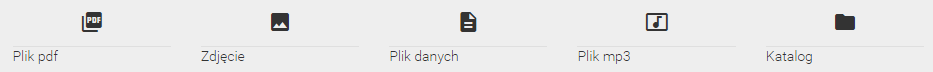
\includegraphics[width=0.7\linewidth]{"obrazy/6.3 Dostepnetypydanych}
	\caption{Dostępne typy danych.}
	\label{datatypes}
\end{figure}


Na wszystkich polach znajdujących się w przestrzeni dyskowej można wykonać operacje używając prawego przycisku myszy. Otworzenie katalogu lub pliku następuje poprzez podwójne wybranie go lewym przyciskiem myszy. Menu kontekstowe może wyświetlić się również dla kliknięcia prawym przyciskiem na przestrzeń nie wykorzystaną przez pliki lub katalogi. Dostępne operacje w menu różnią się. Wszystkie opcje możliwe do wykonania na pliku znajdują się w rysunku \ref{dostOpcje}
\begin{figure}[h!]
	\centering
	\includegraphics[width=0.7\linewidth]{"obrazy/6.3 opcjeplikow"}
	\caption{Dostępne opcje plików.}
	\label{dostOpcje}
\end{figure}

Opcja "Otwórz" wykonana na pliku umożliwi podgląd jego zawartości w panelu bocznym. Dozwolony jest rozwinięcie plików o rozszerzeniu .pdf, docx, doc, mp3, jpg, tiff, jpeg, png. Podgląd innych formatów danych może nie wykonać się pomyślnie.
Operacja "Otwórz" wykonana na folderze umożliwi wyczyszczenie oraz załadowanie danych przestrzeni dyskowej dla danego katalogu. Ponadto do menu lokalizacji zostanie dodany odnośnik wskazujący na folder, w którym użytkownik aktualnie się znajduje. 
\begin{figure}[h!]
	\centering
	\includegraphics[width=0.7\linewidth]{"obrazy/6.3 aktualny katalog"}
	\caption{Stan katalogu po wykonaniu operacji "Otwórz".}
	\label{openDirectory}
\end{figure}

Każdy plik dodany do aplikacji możemy pobrać na dysk twardy. Operacji można dokonać przy użyciu opcji "Pobierz" . Wybranie opcji spowoduje otworzenie eksploratora plików systemu Windows w celu wskazania ścieżki zapisu danych (ewentualnie plik zostanie zapisany w domyślnie wybranym miejscu). Opcja jest dostępna do wykonania na folderach. Uruchomienie jej na katalogu uruchomi pobranie archiwum danych w formacie .zip, w którym znajdywać się będą pliki umieszczone w katalogu. W pobieranych danych zostaną również uwzględnione pozostałe katalogi oraz pliki znajdujące się w nich.

W celu przeniesienia danych do dowolnego folderu należy skorzystać z opcji "Wytnij" lub "Kopiuj" . Operacje można wykonać na dowolnych danych znajdujących się na dysku. Opcja "Kopiuj" przenosi wybrany zasób do dowolnego folderu w przestrzeni. Wykonanie jej spowoduje przetrzymywanie dwóch elementów o tych samych wartościach, w różnej lokalizacji. Opcja "Wytnij" przenosi wybrany zasób do dowolnego miejsca. Operacja ma na celu zmianę lokalizacji danych.

Opcja "Usuń" znajdująca się w menu kontekstowym danych umożliwia usunięcie zasobów z przestrzeni aplikacji. Wybranie jej jest nieodwracalne, a dane nie są możliwe do przywrócenia. Wykonania operacji na katalogu, w którym znajdują się dane, spowoduje usunięcie wszystkich zasobów znajdujących się w nim.

W celu zmiany nazwy pliku lub folderu należy skorzystać z opcji "Zmień nazwę" . Wybranie jej otworzy okno dialogowe z dwoma przyciskami oraz polem przeznaczonym na nową nazwę. Wybranie "Anuluj" spowoduje zamknięcie dialogu. Wpisanie nowej nazwy oraz przyciśnięcie klawisza "Zmień" umożliwi dokonanie operacji. Okno zostało przedstawione w rysunku \ref{ChangeName}

\begin{figure}[!h]
	\centering
	\includegraphics[width=0.7\linewidth]{"obrazy/6.3 ZmianaNazwy"}
	\caption{Okno zmiany nazwy.}
	\label{ChangeName}
\end{figure}

Ostatnią opcją możliwą do wybrania w menu kontekstowym są właściwości. Umożliwiają one podejrzenie informacji o pliku lub folderze. Wybranie opcji spowoduje uruchomienie okna dialogowego z podstawowymi danymi. Użytkownik nie może wpływać na właściwościowi. Okno ma dostępne dwa przyciski służące do zamknięcia go. Rysunek \ref{descriptionWindow} przedstawia właściwości folderu.

\begin{figure}[!h]
	\centering
	\includegraphics[width=0.7\linewidth]{"obrazy/6.3 OknoWlasc"}
	\caption{Okno właściwości.}
	\label{descriptionWindow}
\end{figure}
\newpage
Menu kontekstowe dotyczy nie tylko plików i katalogów, ale również przestrzeni dyskowej. Kliknięcie prawym przyciskiem myszy na przestrzeń, w której nie znajdują się dane spowoduje jego uruchomienie. Menu wyposażone jest w opcje wykonywane na katalogu. Do nich należą operacje: wklej, utwórz folder, odśwież, właściwości oraz dodaj nowe pliki. Menu zostało przedstawione na rysunku \ref{DirectoryMenu}

\begin{figure}[!h]
	\centering
	\includegraphics[width=0.7\linewidth]{"obrazy/6.3 MenuKatalogu"}
	\caption{Menu kontekstowe katalogu.}
	\label{DirectoryMenu}
\end{figure}


